\documentclass[british]{article}
\usepackage[T1]{fontenc}
\usepackage[latin9]{inputenc}
\usepackage{geometry}
\geometry{verbose,tmargin=3.5cm,bmargin=3.5cm,lmargin=3cm,rmargin=3cm}
\usepackage{array}
%\usepackage{multirow}
\usepackage{amstext}
\usepackage{graphicx}
\usepackage{color}
\usepackage[font=small,labelfont=bf]{caption}
%\usepackage{subfigure}

\newcommand{\tabincell}[2]{\begin{tabular}{@{}#1@{}}#2\end{tabular}}

\newcommand{\mytablefontsize}{7pt}
\newcommand{\mytablebaselineskip}{0.7}
\newcommand{\mytabcolsep}{3pt}

\newcommand{\medianInterval}[1]{}

\makeatletter

\newif\iftest
\testtrue

\newif\ifruntime
\runtimetrue

\newif\ifablation
\ablationfalse

\newif\iffeatures
\featuresfalse

%%%%%%%%%%%%%%%%%%%%%%%%%%%%%% LyX specific LaTeX commands.
%% Because html converters don't know tabularnewline
\providecommand{\tabularnewline}{\\}

%%%%%%%%%%%%%%%%%%%%%%%%%%%%%% User specified LaTeX commands.

\title{Configuration Report for the Solver PbO-CCSAT-Generic on the Training Instance Set PTN \iftest and Testing Instance Set PTN2 \fi in \emph{Sparkle} }
\author{ Automatically generated by \emph{Sparkle} (version: 0.8.1) }

\makeatother

\usepackage{babel}
\begin{document}
\maketitle %


\section{Introduction}
\label{sec:Introduction}

\emph{Sparkle} \cite{Hoos15} is a multi-agent problem-solving platform based on Programming by Optimisation (PbO) \cite{Hoos12}, and would provide a number of effective algorithm optimisation techniques (such as automated algorithm configuration, portfolio-based algorithm selection, etc) to accelerate the existing solvers.

This experimental report is automatically generated by \emph{Sparkle}. This report presents experimental results on the scenario of configuring the solver PbO-CCSAT-Generic on the training instance set PTN\iftest~and evaluating it on the testing instance set PTN2\fi.


\section{Information about the Instance Set(s)}

\begin{itemize}
\item Training set: \textbf{PTN}, consisting of 12 instances
\iftest\item Testing set: \textbf{PTN2}, consisting of 11 instances\fi
\end{itemize}


\iffeatures
    \section{Feature Extractors}
        There are @@numFeatureExtractors@@ feature extractor(s) included in \emph{Sparkle}, as listed below.

        \begin{enumerate}
        @@featureExtractorList@@
        \end{enumerate}

        \emph{Sparkle} uses all the feature extractors presented above to compute a feature vector for each training instance. Every feature extractor computes a feature vector for each training instance. The final feature vector is then the combination of all computed feature vectors. The cutoff time for feature vector computation on each training instance is set to @@featureComputationCutoffTime@@ seconds. This time is shared equally between the feature extractors.

        The calculated instance features are then passed on to be used in the process of solver configuration. 

\fi


\section{Information about the Configuration Protocol}

The configurator used in \emph{Sparkle} is SMAC ({\em Sequential Model-based Algorithm Configuration}) \cite{HutEtAl11}, and the version of SMAC used in \emph{Sparkle} is 2.10.03.

During the configuration process, \emph{Sparkle} performs 25 independent SMAC runs for configuring the solver PbO-CCSAT-Generic on the training instance set PTN\iffeatures; the instance features of the training instance set were used for configuration\fi; the configuration objective is RUNTIME; the whole configuration time budget is 600 seconds; the cutoff time for each run is 60 seconds.

Each independent run of SMAC would result in one optimised configuration. As a result, \emph{Sparkle} would obtain 25 optimised configurations. Each of these was then evaluated on the entire training set, with one solver run per instance and a cutoff time of 60 seconds, and the configuration with the lowest PAR10 value was selected as the result of the configuration process.

\section{Information about the Optimised Configuration}

After the configuration process mentioned above, \emph{Sparkle} obtained the optimised configuration. The details of the optimised configuration are described below.

\vspace{5mm}

-p\textunderscore swt '0.37822764235422035' -perform\textunderscore aspiration '1' -perform\textunderscore clause\textunderscore weight '1' -perform\textunderscore double\textunderscore cc '1' -perform\textunderscore first\textunderscore div '0' -perform\textunderscore pac '0' -q\textunderscore swt '0.5433225022192605' -sel\textunderscore clause\textunderscore div '2' -sel\textunderscore clause\textunderscore weight\textunderscore scheme '1' -sel\textunderscore var\textunderscore break\textunderscore tie\textunderscore greedy '1' -sel\textunderscore var\textunderscore div '2' -threshold\textunderscore swt '592'

\vspace{5mm}

%The PAR value of the optimised configuration on the entire training set is 55.45833300000001.

\section{Comparison between Configured Version and Default Version on the Training Instance Set}
In order to investigate the performance on the training instance set, \emph{Sparkle} ran the configured version of PbO-CCSAT-Generic and the default version of PbO-CCSAT-Generic on the training instance set. During this phase, each version performed one run per instance with a cutoff time of 60 seconds. The results are reported as follows.

\begin{itemize}
    \item \textbf{PbO-CCSAT-Generic (configured)}, PAR10: 55.45833300000001
    \item \textbf{PbO-CCSAT-Generic (default)}, PAR10: 226.99671249999997
\end{itemize}

The empirical comparison between the PbO-CCSAT-Generic (configured) and PbO-CCSAT-Generic (default) on the training set of PTN is presented in Figure \ref{fig:configured_vs_default_train}.

\begin{figure}[htbp]
\noindent \begin{centering}
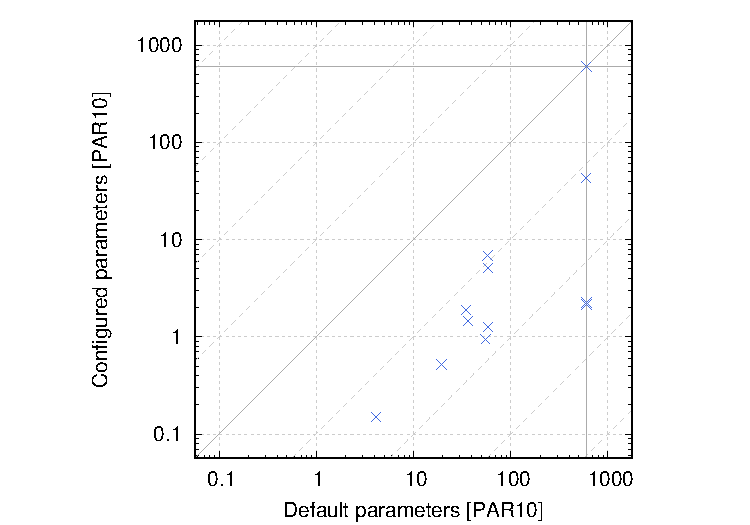
\includegraphics[width=0.6\textwidth]{data_PbO-CCSAT-Generic_configured_vs_default_on_PTN_train}
% \includegraphics[width=0.8\textwidth]{fittedModels}
\par\end{centering}

\caption{Empirical comparison between the PbO-CCSAT-Generic (configured) and PbO-CCSAT-Generic (default) on the training set of PTN.}\label{fig:configured_vs_default_train}
\end{figure}

%\ifruntime

Table \ref{tbl:timeouts_train} shows on how many instances the PbO-CCSAT-Generic (configured) and PbO-CCSAT-Generic (default) timed out (did not solve the instance within the cutoff time of 60 seconds) on the training set of PTN, as well as on how many instances both timed out.

    \begin{table}[htbp]
        \centering
            \begin{tabular}{ccc}
                configured & default & overlap \\ \hline
                1 & 4 & 1
            \end{tabular}
            \caption{Number of time-outs for PbO-CCSAT-Generic (configured), PbO-CCSAT-Generic (default), and for how many instances both timed out on the training set of PTN.}
        \label{tbl:timeouts_train}
    \end{table}

%\fi % End ifruntime

\iftest
    \section{Comparison between Configured Version and Default Version on the Testing Instance Set}

    After specifying the optimised configuration, \emph{Sparkle} ran the configured version of PbO-CCSAT-Generic and the default version of PbO-CCSAT-Generic on the testing instance set. During this phase, each version performed one run per instance with a cutoff time of 60 seconds. The results are reported as follows.

    \begin{itemize}
        \item \textbf{PbO-CCSAT-Generic (configured)}, PAR10: 9.619044545454546
        \item \textbf{PbO-CCSAT-Generic (default)}, PAR10: 130.26663809090908
    \end{itemize}

    The empirical comparison between the PbO-CCSAT-Generic (configured) and PbO-CCSAT-Generic (default) on the testing set of PTN2 is presented in Figure \ref{fig:configured_vs_default_test}.

    \begin{figure}[htbp]
        \noindent
        \begin{centering}
            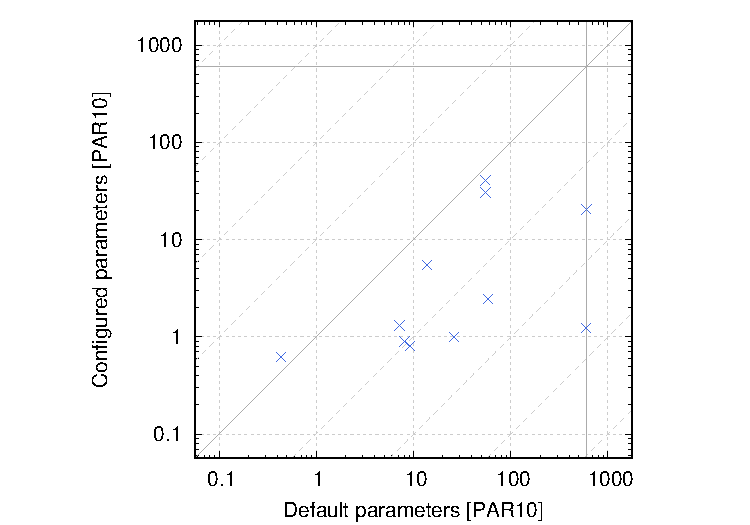
\includegraphics[width=0.6\textwidth]{data_PbO-CCSAT-Generic_configured_vs_default_on_PTN2_test}
            % \includegraphics[width=0.8\textwidth]{fittedModels}
            \par
        \end{centering}

       \caption{Empirical comparison between the PbO-CCSAT-Generic (configured) and PbO-CCSAT-Generic (default) on the testing set of PTN2.}\label{fig:configured_vs_default_test}
    \end{figure}

    %\ifruntime

        Table \ref{tbl:timeouts_test} shows on how many instances the PbO-CCSAT-Generic (configured) and PbO-CCSAT-Generic (default) timed out (did not solve the instance within the cutoff time of 60 seconds) on the testing set of PTN2, as well as on how many instances both timed out.

        \begin{table}[htbp]
            \begin{center}
                \begin{tabular}{ccc}
                    configured & default & overlap \\ \hline
                    0 & 2 & 0
                \end{tabular}
            \end{center}
            \caption{Number of time-outs for PbO-CCSAT-Generic (configured), PbO-CCSAT-Generic (default), and for how many instances both timed out on the testing set of PTN2.}
            \label{tbl:timeouts_test}
        \end{table}

    %\fi % End ifruntime

\fi % End iftest

\ifablation
    \section{Parameter importance via Ablation}

    Ablation analysis~\cite{FawcettHoos16} is performed from the PbO-CCSAT-Generic (default) to PbO-CCSAT-Generic (configured) to see which parameter changes between them contribute most to the improved performance.
    \iftest
    The ablation path uses the training set PTN and validation is perform on the test set PTN2.
    \else
    The ablation path is constructed and validated with the training set PTN.
    \fi
    The set of parameters that differ in the two configurations will form the ablation path.
    Starting from the default configuration, the path is computed by performing a sequence of rounds.
    In a round, each available parameter is flipped in the configuration and is validated on its performance.
    The flipped parameter with the best performance in that round, is added to the configuration and the next round starts with the remaining parameters.
    This repeats until all parameters are flipped, which is the best found configuration.
    The analysis resulted in the ablation path presented in Table~\ref{table:ablationpath}.


    \begin{table}[htbp]
        \caption{Ablation path from PbO-CCSAT-Generic (default) to PbO-CCSAT-Generic (configured) where parameters with higher importance are ranked higher.}
        \label{table:ablationpath}
        \begin{center}
        \footnotesize
            \begin{tabular}{rp{0.25\linewidth}rrr}\end{tabular}
        \end{center}
    \end{table}

\fi % End ablation

\bibliographystyle{plain}
\bibliography{/home/snelleman/Sparkle/Components/Sparkle-latex-source/SparkleReport.bib}

\end{document}
